\chapter{Testing Result}
\label{ch:AccuracyResult}

This section shows the detail test result of each algorithm.

\section{Linear Regression}

The result of linear regression are shown in figure~\ref{fg:lrCdc}, \ref{fg:lrMape} and \ref{fg:lrMse}. Linear regression is a good algorithm, with the fastest speed and a relatively good performance. Its average CDC is around 50.79\%, mean MSE is 2.83 and mean MAPE is 2.01\%.

\begin{figure}[h]
	\centering
	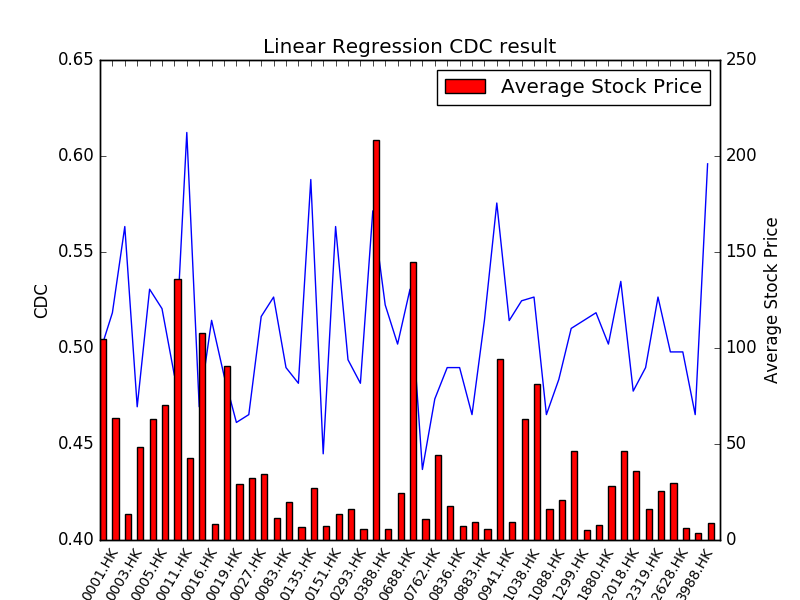
\includegraphics[width=0.8\textwidth]{TestingResult/LRCDC}
	\caption{Linear Regression CDC result}
	\label{fg:lrCdc}
\end{figure}

\begin{figure}[h]
	\centering
	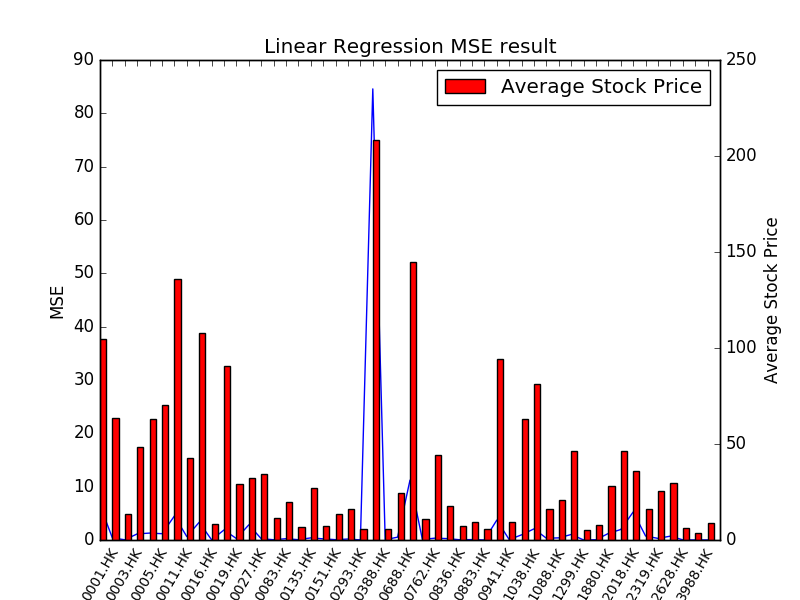
\includegraphics[width=0.8\textwidth]{TestingResult/LRMSE}
	\caption{Linear Regression MSE result}
	\label{fg:lrMse}
\end{figure}

\begin{figure}[h]
	\centering
	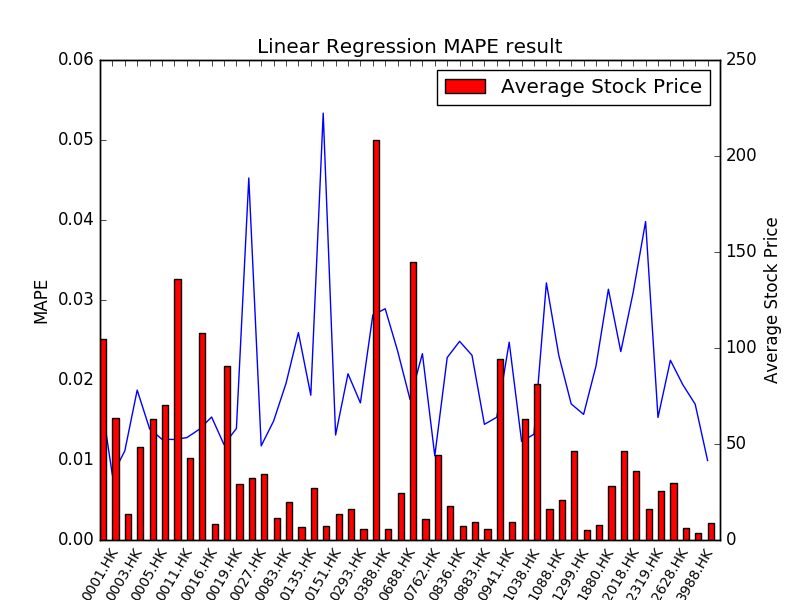
\includegraphics[width=0.8\textwidth]{TestingResult/LRMAPE}
	\caption{Linear Regression MAPE result}
	\label{fg:lrMape}
\end{figure}

\clearpage

\section{Random Forest}

The result of random forest are shown in figure~\ref{fg:rtCdc}, \ref{fg:rtMape} and \ref{fg:rtMse}. Its average CDC is around 49.27\%, mean MSE is 90.99 and mean MAPE is 9.15\%.

\begin{figure}[h]
	\centering
	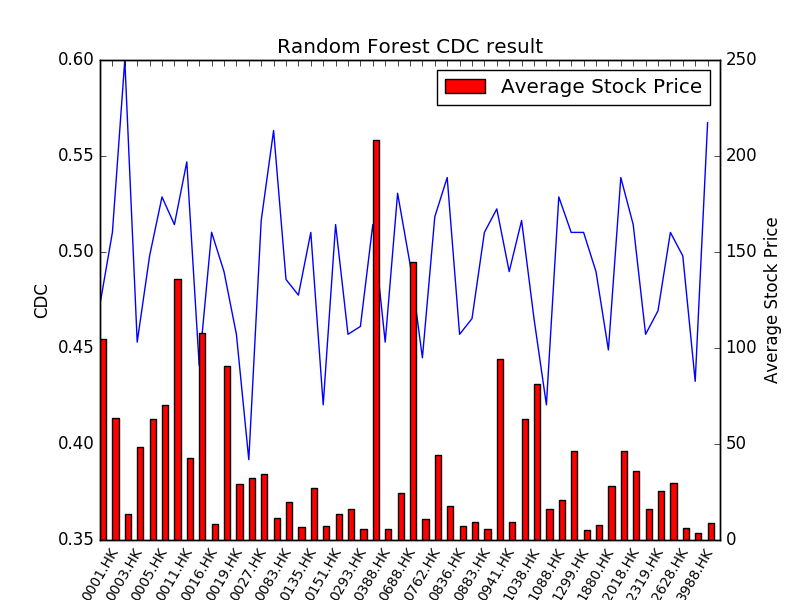
\includegraphics[width=0.8\textwidth]{TestingResult/RFCDC}
	\caption{Random Forest CDC result}
	\label{fg:rtCdc}
\end{figure}

\begin{figure}[h]
	\centering
	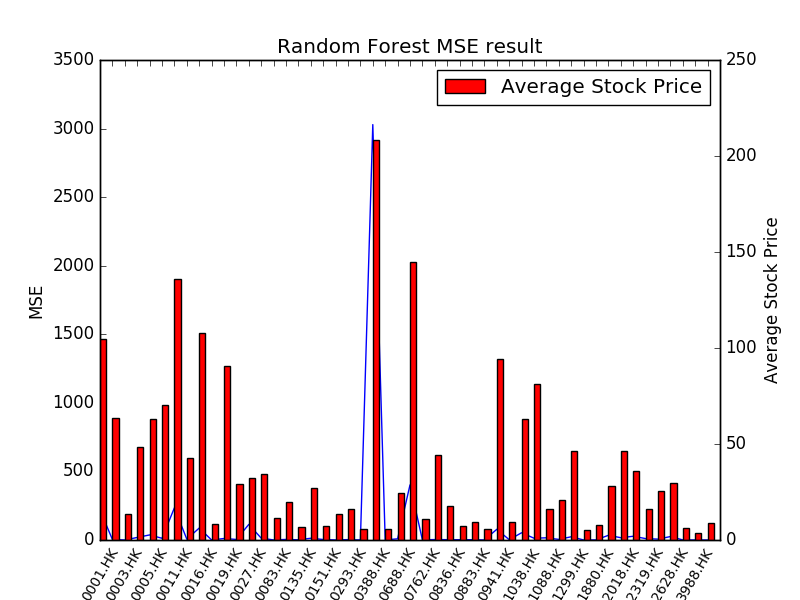
\includegraphics[width=0.8\textwidth]{TestingResult/RFMSE}
	\caption{Random Forest MSE result}
	\label{fg:rtMse}
\end{figure}

\begin{figure}[h]
	\centering
	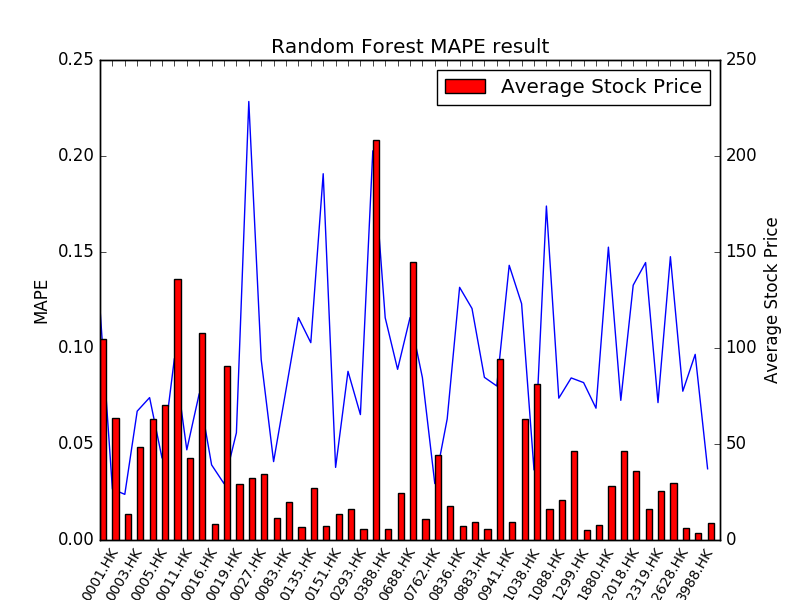
\includegraphics[width=0.8\textwidth]{TestingResult/RFMAPE}
	\caption{Random Forest MAPE result}
	\label{fg:rtMape}
\end{figure}

\clearpage

\section{Artificial Neural Network}

The result of ANN are shown in figure~\ref{fg:annCdc}, \ref{fg:annMape} and \ref{fg:annMse}. Its average CDC is around 48.73\%, mean MSE is 183.69 and mean MAPE is 15.87\%.

\begin{figure}[h]
	\centering
	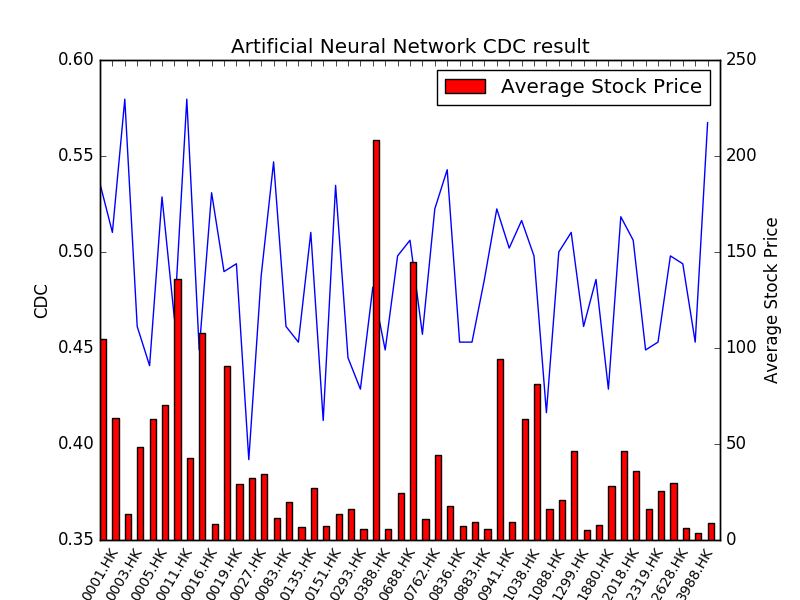
\includegraphics[width=0.8\textwidth]{TestingResult/ANNCDC}
	\caption{Artificial Neural Network CDC result}
	\label{fg:annCdc}
\end{figure}

\begin{figure}[h]
	\centering
	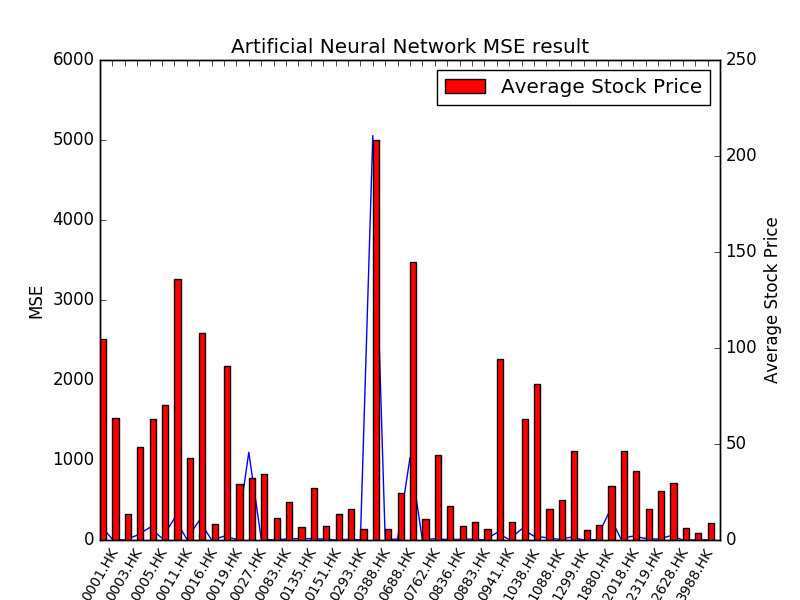
\includegraphics[width=0.8\textwidth]{TestingResult/ANNMSE}
	\caption{Artificial Neural Network MSE result}
	\label{fg:annMse}
\end{figure}

\begin{figure}[h]
	\centering
	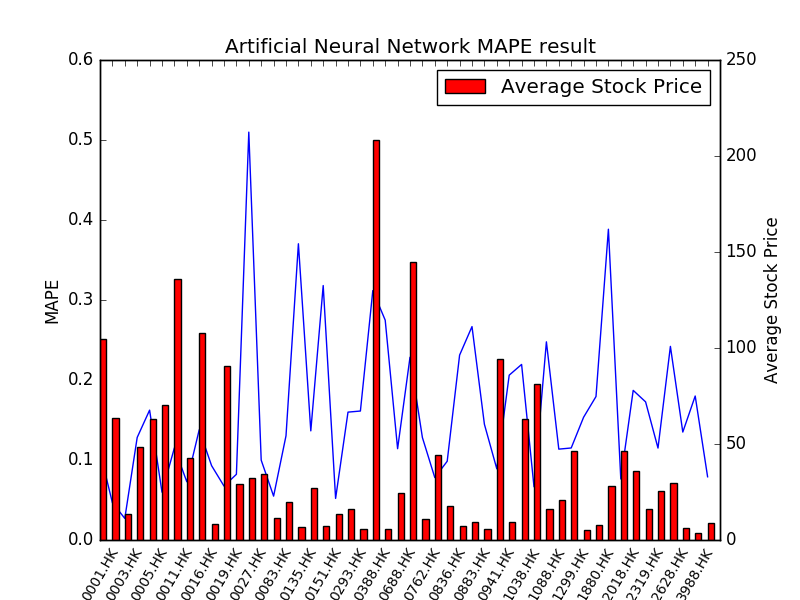
\includegraphics[width=0.8\textwidth]{TestingResult/ANNMAPE}
	\caption{Artificial Neural Network MAPE result}
	\label{fg:annMape}
\end{figure}

\clearpage

\section{Artificial Neural Network + Artificial Neural Network}

This system consists of two methods, using ANN as classifier and another use it as regressor. Its results are shown in figure~\ref{fg:annAnnCdc}, \ref{fg:annAnnMape} and \ref{fg:annAnnMse}. Its average CDC is around 50.10\%, mean MSE is 16.61 and mean MAPE is 5.59\%.

\begin{figure}[h]
	\centering
	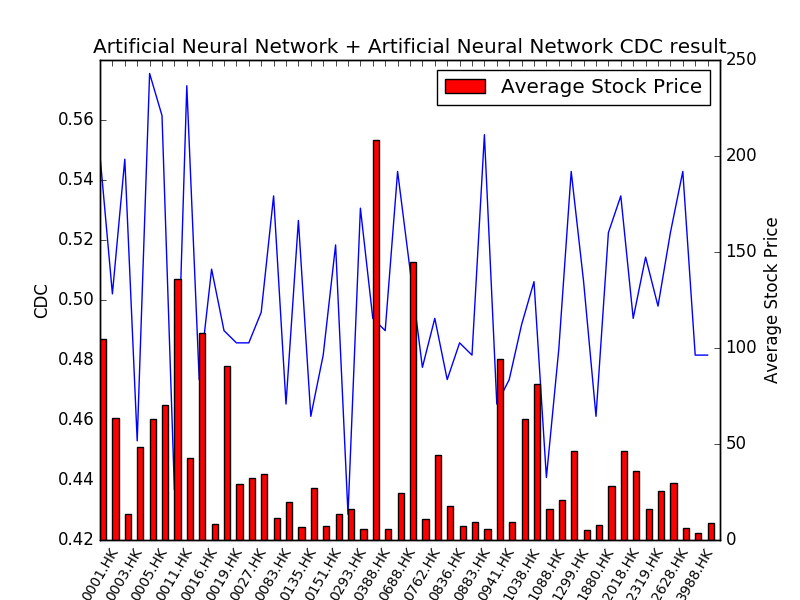
\includegraphics[width=0.8\textwidth]{TestingResult/ANN+ANNCDC}
	\caption{Artificial Neural Network + Artificial Neural Network CDC result}
	\label{fg:annAnnCdc}
\end{figure}

\begin{figure}[h]
	\centering
	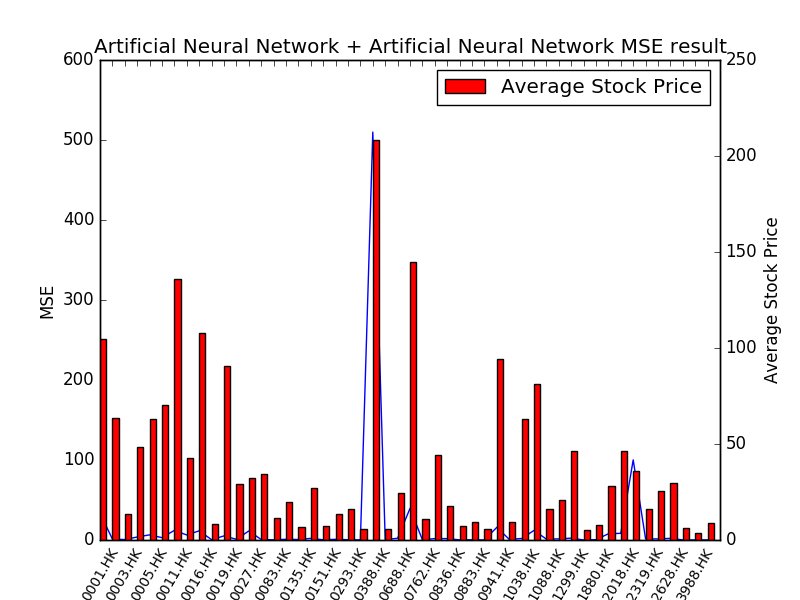
\includegraphics[width=0.8\textwidth]{TestingResult/ANN+ANNMSE}
	\caption{Artificial Neural Network + Artificial Neural Network MSE result}
	\label{fg:annAnnMse}
\end{figure}

\begin{figure}[h]
	\centering
	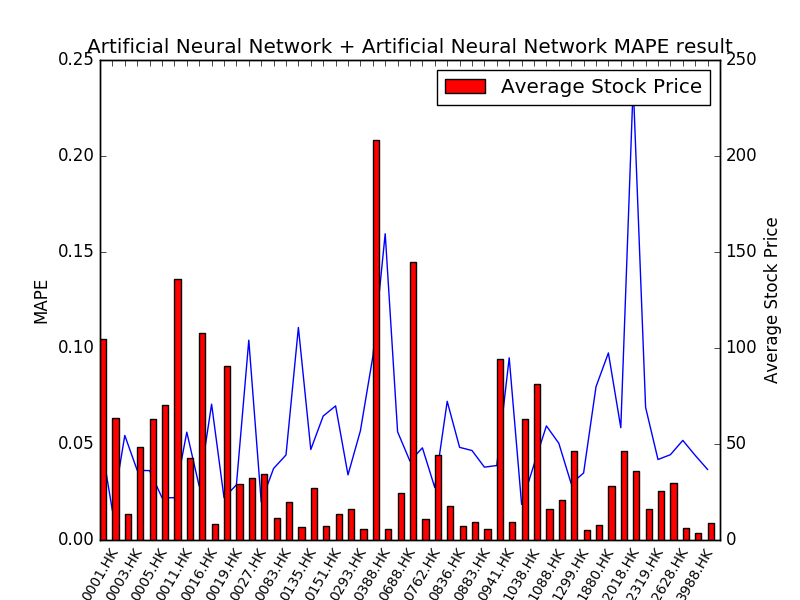
\includegraphics[width=0.8\textwidth]{TestingResult/ANN+ANNMAPE}
	\caption{Artificial Neural Network + Artificial Neural Network MAPE result}
	\label{fg:annAnnMape}
\end{figure}

\clearpage


\section{Random Forest + Linear Regression}

This system consists of two methods, using Random Forest as classifier to predict stock change direction and use Linear Regression as regressor. Its results are shown in figure~\ref{fg:rfLrCdc}, \ref{fg:rfLrMape} and \ref{fg:rfLrMse}. Its average CDC is around 50.10\%, mean MSE is 16.61 and mean MAPE is 5.59\%.

\begin{figure}[h]
	\centering
	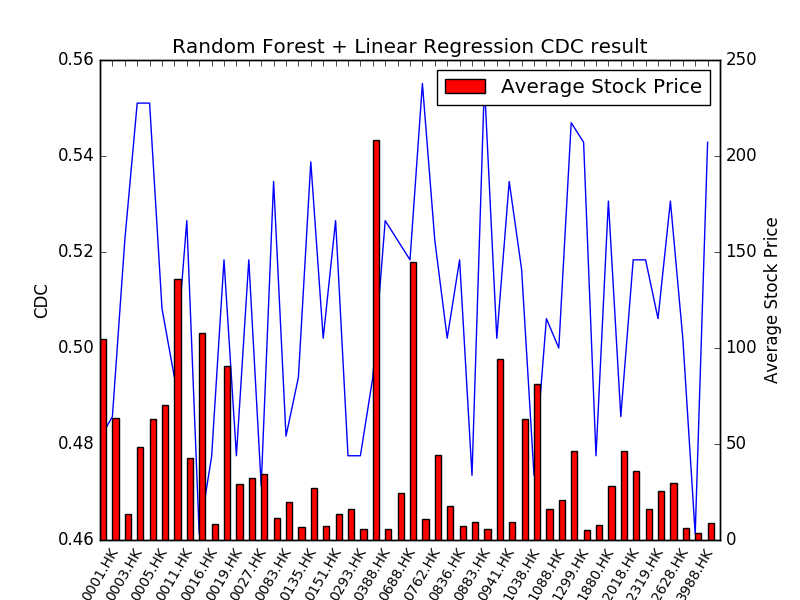
\includegraphics[width=0.8\textwidth]{TestingResult/RF+LRCDC}
	\caption{Random Forest + Linear Regression CDC result}
	\label{fg:rfLrCdc}
\end{figure}

\begin{figure}[h]
	\centering
	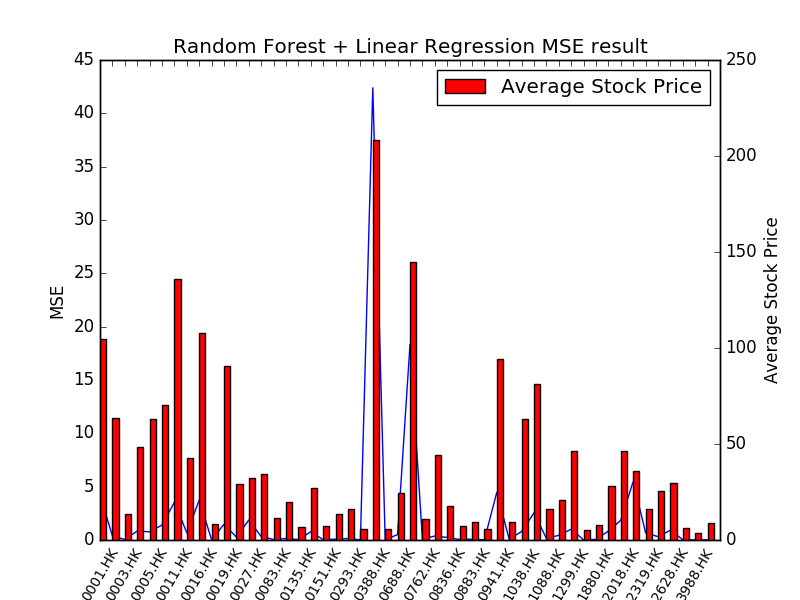
\includegraphics[width=0.8\textwidth]{TestingResult/RF+LRMSE}
	\caption{Random Forest + Linear Regression MSE result}
	\label{fg:rfLrMse}
\end{figure}

\begin{figure}[h]
	\centering
	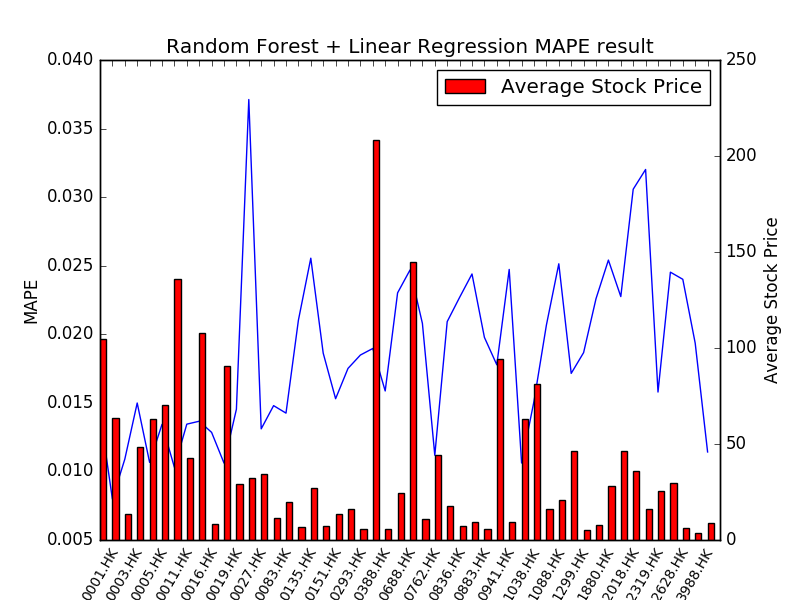
\includegraphics[width=0.8\textwidth]{TestingResult/RF+LRMAPE}
	\caption{Random Forest + Linear Regression MAPE result}
	\label{fg:rfLrMape}
\end{figure}

\clearpage

\section{Logistic Regression + Random Forest}

This system consists of two methods, using Logistic Regression as classifier to predict stock change direction and use Random Forest as regressor to predict stock change amount. Its results are shown in figure~\ref{fg:lrRfCdc}, \ref{fg:lrRfMape} and \ref{fg:lrRfMse}. Its average CDC is around 50.32\%, mean MSE is 2.79 and mean MAPE is 2.30\%.

\begin{figure}[h]
	\centering
	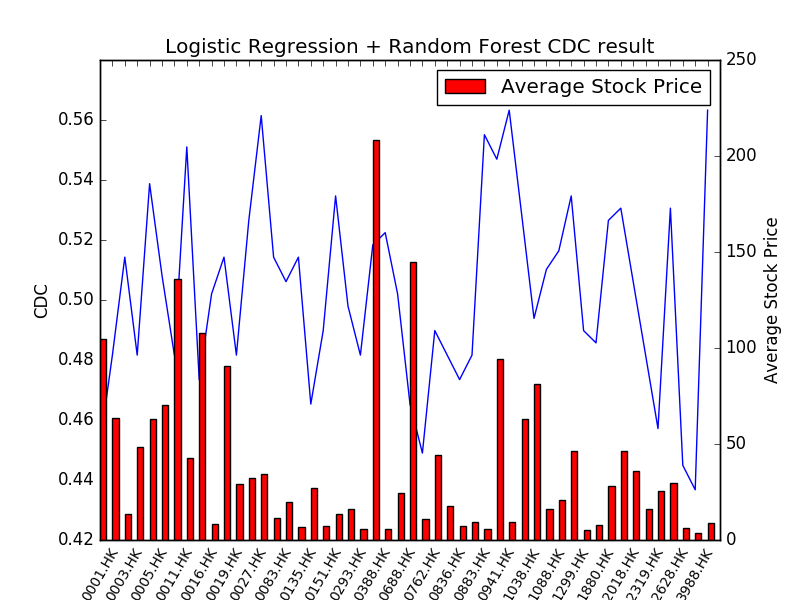
\includegraphics[width=0.8\textwidth]{TestingResult/LR+RFCDC}
	\caption{Logistic Regression + Random Forest CDC result}
	\label{fg:lrRfCdc}
\end{figure}

\begin{figure}[h]
	\centering
	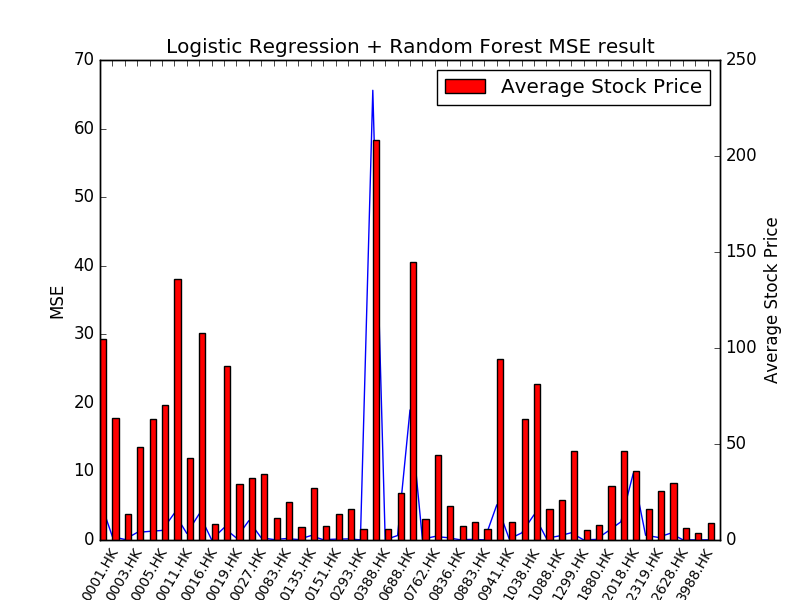
\includegraphics[width=0.8\textwidth]{TestingResult/LR+RFMSE}
	\caption{Logistic Regression + Random Forest MSE result}
	\label{fg:lrRfMse}
\end{figure}

\begin{figure}[h]
	\centering
	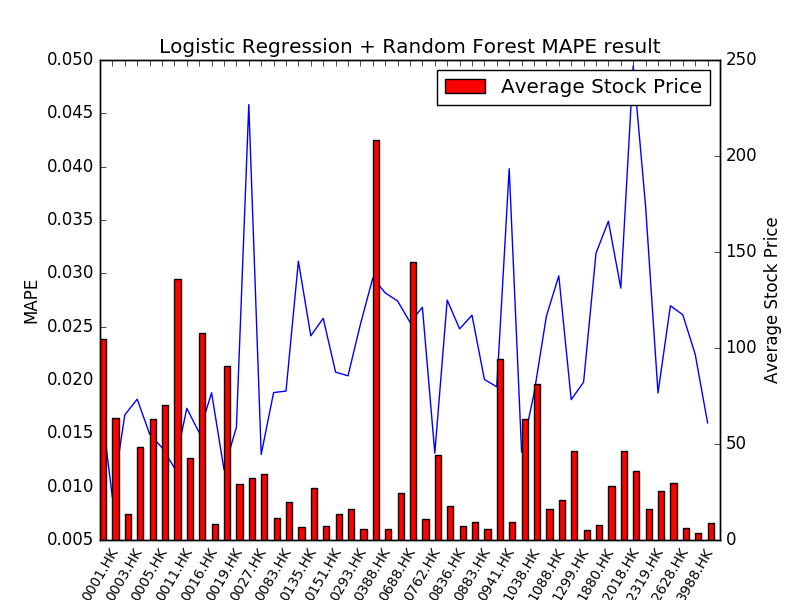
\includegraphics[width=0.8\textwidth]{TestingResult/LR+RFMAPE}
	\caption{Logistic Regression + Random Forest MAPE result}
	\label{fg:lrRfMape}
\end{figure}

\clearpage

\section{Summary}

The average results are shown in table~\ref{tb:averageResult}. Form this table we can find that use random forest as classifier and linear regression as regressor can achieve the best performance.

\begin{table}[h]
	\centering
	\begin{tabular}{|c|c|c|c|c|}
		\hline
		& \textbf{CDC}     & \textbf{MSE}  & \textbf{MAPE}   & \textbf{Run Time} \\ \hline
		\textbf{LR}        & 50.79\%          & 2.83          & 2.01\%          & \textbf{9.74}     \\ \hline
		\textbf{RF}        & 49.27\%          & 90.99         & 9.15\%          & 17.32             \\ \hline
		\textbf{ANN}       & 48.73\%          & 183.69        & 15.87\%         & 15.82             \\ \hline
		\textbf{ANN + ANN} & 50.10\%          & 16.31         & 5.59\%          & 26.87             \\ \hline
		\textbf{LogR + RF} & 50.32\%          & 2.79          & 2.30\%          & 19.92             \\ \hline
		\textbf{RF + LinR} & \textbf{50.92\%} & \textbf{2.05} & \textbf{1.85\%} & 13.10             \\ \hline
	\end{tabular}
	\caption{Test result of different learning algorithm.}
	\label{tb:averageResult}
\end{table}